% Options for packages loaded elsewhere
\PassOptionsToPackage{unicode}{hyperref}
\PassOptionsToPackage{hyphens}{url}
%
\documentclass[
]{article}
\usepackage{amsmath,amssymb}
\usepackage{iftex}
\ifPDFTeX
  \usepackage[T1]{fontenc}
  \usepackage[utf8]{inputenc}
  \usepackage{textcomp} % provide euro and other symbols
\else % if luatex or xetex
  \usepackage{unicode-math} % this also loads fontspec
  \defaultfontfeatures{Scale=MatchLowercase}
  \defaultfontfeatures[\rmfamily]{Ligatures=TeX,Scale=1}
\fi
\usepackage{lmodern}
\ifPDFTeX\else
  % xetex/luatex font selection
\fi
% Use upquote if available, for straight quotes in verbatim environments
\IfFileExists{upquote.sty}{\usepackage{upquote}}{}
\IfFileExists{microtype.sty}{% use microtype if available
  \usepackage[]{microtype}
  \UseMicrotypeSet[protrusion]{basicmath} % disable protrusion for tt fonts
}{}
\makeatletter
\@ifundefined{KOMAClassName}{% if non-KOMA class
  \IfFileExists{parskip.sty}{%
    \usepackage{parskip}
  }{% else
    \setlength{\parindent}{0pt}
    \setlength{\parskip}{6pt plus 2pt minus 1pt}}
}{% if KOMA class
  \KOMAoptions{parskip=half}}
\makeatother
\usepackage{xcolor}
\usepackage[margin=1in]{geometry}
\usepackage{graphicx}
\makeatletter
\def\maxwidth{\ifdim\Gin@nat@width>\linewidth\linewidth\else\Gin@nat@width\fi}
\def\maxheight{\ifdim\Gin@nat@height>\textheight\textheight\else\Gin@nat@height\fi}
\makeatother
% Scale images if necessary, so that they will not overflow the page
% margins by default, and it is still possible to overwrite the defaults
% using explicit options in \includegraphics[width, height, ...]{}
\setkeys{Gin}{width=\maxwidth,height=\maxheight,keepaspectratio}
% Set default figure placement to htbp
\makeatletter
\def\fps@figure{htbp}
\makeatother
\setlength{\emergencystretch}{3em} % prevent overfull lines
\providecommand{\tightlist}{%
  \setlength{\itemsep}{0pt}\setlength{\parskip}{0pt}}
\setcounter{secnumdepth}{-\maxdimen} % remove section numbering
\ifLuaTeX
  \usepackage{selnolig}  % disable illegal ligatures
\fi
\IfFileExists{bookmark.sty}{\usepackage{bookmark}}{\usepackage{hyperref}}
\IfFileExists{xurl.sty}{\usepackage{xurl}}{} % add URL line breaks if available
\urlstyle{same}
\hypersetup{
  pdftitle={Predicting and Analyzing College Student Lifestyle and Spending Patterns in Major Cities of Saudi Arabia},
  hidelinks,
  pdfcreator={LaTeX via pandoc}}

\title{Predicting and Analyzing College Student Lifestyle and Spending
Patterns in Major Cities of Saudi Arabia}
\author{}
\date{\vspace{-2.5em}}

\begin{document}
\maketitle

{
\setcounter{tocdepth}{3}
\tableofcontents
}
\hypertarget{introduction}{%
\section{Introduction:}\label{introduction}}

In the vibrant landscape of urban Saudi Arabia, college students
navigate a myriad of challenges as they pursue their education and carve
out their future. Balancing academic commitments with financial
constraints and lifestyle choices, these students embody the complex
interplay of ambition, culture, and socioeconomic factors. This research
embarks on a crucial exploration, aiming to unravel the underlying
patterns that influence the spending habits and lifestyle choices of
college students in major Saudi cities.

The primary aim of this project is to gain profound insights into the
financial behaviors of college students in urban Saudi environments. We
seek to understand the diverse factors, including gender, age, study
year, socioeconomic background, and individual habits, that impact
students' spending patterns. By delving deep into these intricacies, we
aim to unravel the unique challenges faced by students, providing a
nuanced understanding of their financial decisions within the cultural
context of Saudi Arabia.

Our goals are to uncover patterns- identify recurring patterns and
trends in students' spending habits, shedding light on the factors
driving these behaviors-, inform support systems- provide actionable
insights for educational institutions and policymakers to design
targeted support systems, addressing the specific needs of students-,
and enhance student experience- facilitate businesses catering to
students in tailoring their services, ensuring they align with authentic
student needs and preferences.

In this report, we will meticulously analyze the dataset, employing
various statistical and machine learning techniques to derive meaningful
conclusions. We will offer a comprehensive roadmap of our analysis,
encompassing data collection, preprocessing, modeling, and
interpretation of results. Through detailed visualizations and clear
explanations, we aim to present a cohesive narrative of our findings,
allowing readers to grasp the complexities of student financial
behaviors in Saudi urban environments.

\hypertarget{significance-and-problem-statement}{%
\section{Significance and Problem
Statement:}\label{significance-and-problem-statement}}

The project addresses the fundamental issue of understanding the
financial dynamics of college students in urban Saudi settings. While
prior studies have explored similar themes on a global scale, there
exists a dearth of research focusing specifically on the nuanced context
of Saudi Arabian students within their local cities. This project
bridges this gap by conducting a light literature review, summarizing
existing works related to student spending behaviors and lifestyle
choices. By drawing on this background, we contextualize our analysis,
laying the foundation for our exploration into the unique challenges
faced by students in major Saudi cities.

\hypertarget{literature-review}{%
\section{Literature Review}\label{literature-review}}

Prior research has explored the financial behaviors of college students
on a global scale, providing valuable insights into the challenges and
dynamics of student spending. However, within the specific context of
urban Saudi Arabia, there is a notable dearth of studies focusing on the
nuanced intricacies of students' financial decisions. This light
literature review aims to highlight key themes and findings from
existing research, setting the stage for our exploration into the unique
challenges faced by college students in major Saudi cities.

\hypertarget{financial-behavior-of-saudi-college-students}{%
\subsection{Financial Behavior of Saudi College
Students}\label{financial-behavior-of-saudi-college-students}}

Research specifically focusing on Saudi college students' financial
behaviors is limited but growing. (Ali Saleh Alshebami \& Theyazn H. H.
Aldhyani, 2022) provides a foundational look into the spending habits of
Saudi students, indicating a trend towards consumerism influenced by
social circles and family support. This is echoed by the fac that
financial support from families often dictates the spending habits and
lifestyle choices of students in Saudi Arabia.

\hypertarget{the-role-of-financial-education}{%
\subsection{The Role of Financial
Education}\label{the-role-of-financial-education}}

In Saudi Arabia, the perceived need for financial education among
college students is gaining attention. (Saeed, 2014) argue that the lack
of formal financial education in the Saudi education system could lead
to poor financial decisions among youths. This gap in the education
system highlights the need for initiatives that can bolster financial
literacy, particularly as the country's economy diversifies under Vision
2030.

\hypertarget{socioeconomic-background-and-spending-patterns}{%
\subsection{Socioeconomic Background and Spending
Patterns}\label{socioeconomic-background-and-spending-patterns}}

The relationship between socioeconomic status and spending behavior is a
critical area of study. (Hamdan, Sue L.T. Mcgregor, \& Elhassan, 2021)
explored this within the Saudi context, finding that students from
higher socioeconomic backgrounds tend to exhibit more significant
consumerist behaviors. These patterns are also influenced by the rapidly
changing retail landscape in urban areas, as discussed by (Otaibi \&
Kausar Yasmeen, 2014), who highlighted the proliferation of malls and
luxury goods as a factor in student spending.

\hypertarget{cultural-influences-on-financial-behavior}{%
\subsection{Cultural Influences on Financial
Behavior}\label{cultural-influences-on-financial-behavior}}

Saudi Arabia's cultural norms and values exert a strong influence on
spending habits. (Alsahafi \& Shin, 2017) examined how cultural
expectations, particularly around events and social gatherings, can lead
to increased expenditure among college students. The pressure to
maintain social status through material possessions is particularly
pronounced in urban centers where there is greater exposure to luxury
and consumerist lifestyles.

\hypertarget{lifestyle-choices-and-expenditure-patterns}{%
\subsection{Lifestyle Choices and Expenditure
Patterns}\label{lifestyle-choices-and-expenditure-patterns}}

The lifestyle choices of Saudi college students, including leisure
activities, dining out, and travel, are influenced by a combination of
globalized cultural trends and local traditions (Qahwaji, 2023).(Al \&
Abu, 2023) highlight how the pursuit of a modern lifestyle among
students in urban centers can lead to increased discretionary spending.

\hypertarget{cultural-and-familial-influence}{%
\subsection{Cultural and Familial
Influence}\label{cultural-and-familial-influence}}

Saudi society maintains strong familial ties, and this extends into the
financial behaviors of college students. (Al-Rethaiaa, Fahmy, \&
Alshwaiyat, 2010) suggests that family allowances are the primary source
of income for many students, which can lead to a lack of financial
autonomy and experience in managing personal finances. The cultural
emphasis on generosity and hospitality can also lead to increased social
spending.

In conclusion, our literature review has laid a foundational
understanding of the existing knowledge on college student lifestyle and
spending patterns, particularly within major cities of Saudi Arabia.
Through scrutinizing various studies, we've identified key factors that
influence these patterns and have revealed a substantial gap in
localized research. This synthesis will serve as a cornerstone for our
own analysis, allowing for a more tailored approach to understanding and
predicting the behaviors of Saudi college students. The insights derived
from our review will guide the methodology of our primary research and
ensure that it is grounded in a robust theoretical framework.

\hypertarget{global-perspective}{%
\subsection{Global Perspective:}\label{global-perspective}}

Numerous studies have delved into the financial behaviors of college
students worldwide, revealing common themes such as the impact of
socioeconomic background, academic pressures, and lifestyle choices on
spending habits. Research by Rehr et al identified a strong correlation
between financial stress and academic performance, emphasizing the need
for targeted support systems (Rehr et al., 2022).

\hypertarget{regional-variances}{%
\subsection{Regional Variances:}\label{regional-variances}}

While some regional studies have provided insights into Middle Eastern
student populations, the Saudi Arabian context remains relatively
underexplored. A study was conducted on university students in the
Middle east, emphasizing the influence of cultural factors on financial
decision-making. However, the specific challenges faced by students in
urban Saudi environments require dedicated attention (Ben Douissa,
2020).

\hypertarget{research-gap}{%
\subsection{Research Gap:}\label{research-gap}}

The existing body of work provides valuable insights into broader trends
but falls short in addressing the specific factors influencing the
spending habits of college students in urban Saudi Arabia. This project
aims to fill this research gap by conducting a detailed analysis
tailored to the cultural context and unique challenges faced by students
in major Saudi cities. Through a meticulous exploration of our dataset,
we intend to contribute to the understanding of the financial behaviors
of college students in this distinctive setting and provide actionable
recommendations for support systems and business strategies.

\hypertarget{data}{%
\section{Data}\label{data}}

\hypertarget{source-of-survey-questions}{%
\subsection{Source of Survey
Questions:}\label{source-of-survey-questions}}

The survey instrument used in this study is adapted from a previous
research project, with questions specifically tailored to the context of
Saudi universities. The original set of questions served as a
foundational framework, and modifications were made to ensure relevance
and cultural appropriateness within the Saudi context.

\hypertarget{unit-of-observation}{%
\subsection{Unit of Observation:}\label{unit-of-observation}}

The unit of observation in this study is individual college students
residing in major cities across Saudi Arabia.

\hypertarget{outcome-variable}{%
\subsection{Outcome Variable:}\label{outcome-variable}}

Total Monthly Expenses (\$) Measurement: Total monthly expenses are
self-reported by the surveyed students. Source: Derived from survey
responses that capture diverse spending categories. Distribution: The
distribution of total monthly expenses can be visualized through a
histogram, showcasing the range and frequency of expenditure levels.

\begin{figure}
\centering
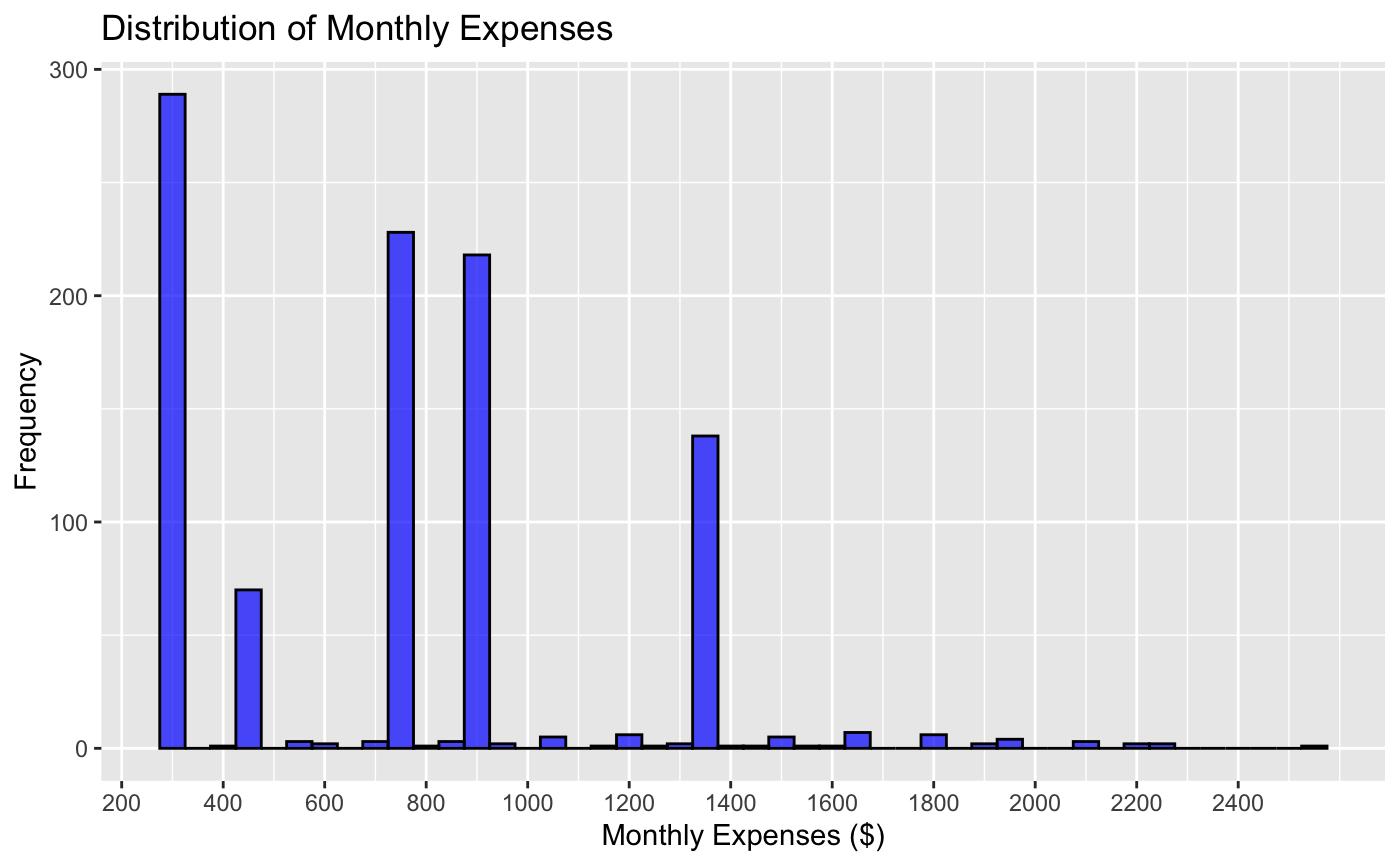
\includegraphics{Distribution_of_Monthly_Expenses.png}
\caption{Distribution of Monthly Expenses Amoung Participants}
\end{figure}

\hypertarget{predictor-variables}{%
\subsection{Predictor Variables:}\label{predictor-variables}}

\begin{enumerate}
\def\labelenumi{\arabic{enumi}.}
\tightlist
\item
  Gender Measurement: Categorical variable (Male, Female, Other).
  Source: Self-reported in the survey.
\item
  Age Measurement: Continuous variable indicating the age of the
  student. Source: Self-reported in the survey.
\item
  Study Year Measurement: Categorical variable (e.g., Freshman,
  Sophomore, Junior, Senior). Source: Self-reported in the survey.
\item
  Socioeconomic Background Measurement: Composite variable based on
  factors like parental income, employment status, and education level.
  Source: Self-reported in the survey.
\end{enumerate}

\begin{figure}
\centering
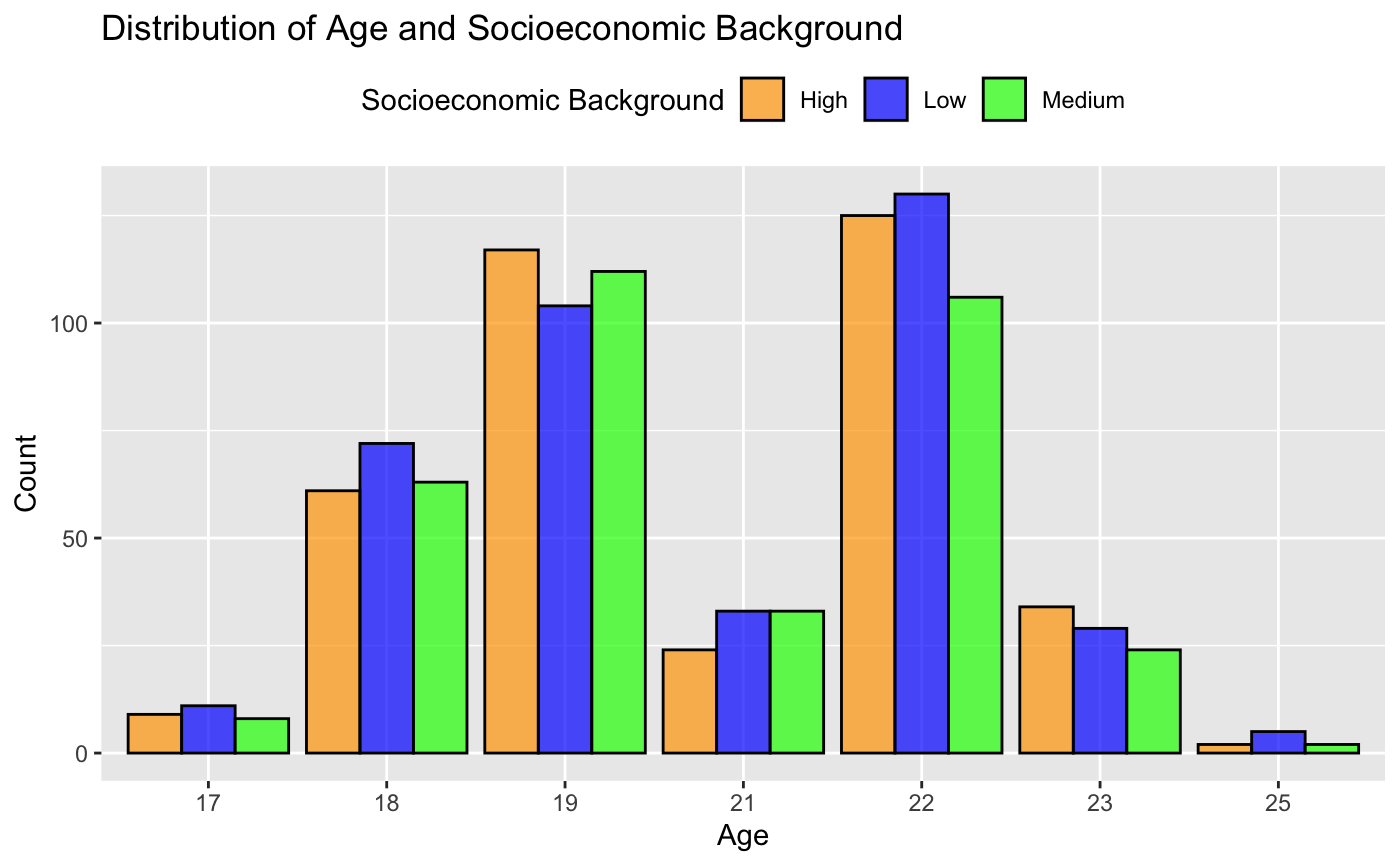
\includegraphics{Distribution_of_Age_and_Socioeconomic_Background.png}
\caption{Distribution of Age and Socioeconomic Background Amoung
Participants}
\end{figure}

\hypertarget{potential-issues-with-the-data}{%
\subsection{Potential Issues with the
Data:}\label{potential-issues-with-the-data}}

Missingness: Addressed through imputation techniques to fill in missing
values. Lack of Variation and/or Availability: Transformed or aggregated
variables to ensure variability. Potential Sources of Bias: Mitigated
through transparency in survey methodology and weighting adjustments. o
How do you overcome/mitigate these issues in your analysis?

\hypertarget{methods-and-tools-exploration}{%
\section{Methods and Tools
Exploration}\label{methods-and-tools-exploration}}

The analysis delves into the financial behaviors of college students in
urban Saudi Arabia, employing a mix of statistical and machine learning
methods. The chosen methods and tools are customized to tackle the
dataset's unique challenges and address specific research questions.

\hypertarget{data-collection-and-preprocessing}{%
\subsection{Data Collection and
Preprocessing}\label{data-collection-and-preprocessing}}

\begin{enumerate}
\def\labelenumi{\alph{enumi}.}
\tightlist
\item
  Loading Data: The dataset is imported into the R environment using the
  readxl package, specifically designed to suit the Saudi cultural
  context.
\item
  Data Cleaning: Key steps involve converting relevant columns to
  numeric formats and handling missing or zero values, ensuring data
  integrity for subsequent analyses.
\item
  Exploratory Data Analysis (EDA): Initial exploration includes an
  overview of the dataset's structure, checking for missing values, and
  utilizing visualizations to comprehend variable distributions and
  relationships.
\end{enumerate}

\hypertarget{feature-selection-and-predictor-variables}{%
\subsection{Feature Selection and Predictor
Variables}\label{feature-selection-and-predictor-variables}}

\begin{enumerate}
\def\labelenumi{\alph{enumi}.}
\tightlist
\item
  Outcome Variable: The primary focus is on `Total Monthly Expenses
  (\$),' elucidated through histograms to showcase its distribution.
\item
  Predictor Variables: Meticulously curated from a published paper,
  these include gender, age, study year, living arrangements,
  socioeconomic background, and various lifestyle choices, providing a
  comprehensive understanding of students' spending patterns. \#\#
  Machine Learning Models
\item
  Random Forest Regression: Utilized for its ability to capture
  non-linear relationships and handle both numerical and categorical
  predictors. It proves suitable for exploring complex patterns within
  the dataset.
\item
  Gradient Boosting Regression: Employed for its effectiveness in
  capturing intricate patterns and interactions among variables,
  enhancing predictive accuracy.
\item
  Linear Regression: Applied as a benchmark model for comparison,
  providing insights into linear relationships between predictors and
  the outcome variable.
\item
  Support Vector Machine (SVM): Chosen for its versatility in handling
  both linear and non-linear relationships, contributing to a
  comprehensive understanding of the data.
\end{enumerate}

\hypertarget{justification-of-toolsmethods}{%
\subsection{Justification of
Tools/Methods}\label{justification-of-toolsmethods}}

Understanding and predicting monthly expenses among college students in
urban Saudi Arabia is a multifaceted task, influenced by various factors
and behaviors. To address this challenge, a repertoire of regression
models was considered: Random Forest regression, Linear Regression,
Support Vector Machine (SVM), and Gradient Boosting Regression. Each
method was chosen for its unique capabilities, aiming to capture the
nuanced relationships between predictors and monthly expenses.

\begin{enumerate}
\def\labelenumi{\arabic{enumi}.}
\tightlist
\item
  Random Forest regression
\end{enumerate}

For predicting monthly expenses among college students in urban Saudi
Arabia, a Random Forest regression model was chosen due to its
robustness in handling complex datasets, non-parametric nature, ability
to capture nonlinear relationships, and feature importance
estimation.The Random Forest regression model was trained on a portion
of the dataset and evaluated using various metrics to assess its
predictive performance on unseen data.

\begin{enumerate}
\def\labelenumi{\arabic{enumi}.}
\setcounter{enumi}{1}
\tightlist
\item
  Linear Regression
\end{enumerate}

The choice of Linear Regression for predicting monthly expenses among
college students was driven by its simplicity, interpretability, and
suitability for capturing linear relationships between predictors and
the target variable. Interpretability: Linear Regression allows easy
interpretation of coefficients, enabling insights into the impact of
each predictor variable on monthly expenses.Baseline Model: Often used
as a baseline model in regression tasks, Linear Regression provides a
fundamental understanding of predictive performance before employing
more complex models

\begin{enumerate}
\def\labelenumi{\arabic{enumi}.}
\setcounter{enumi}{2}
\tightlist
\item
  SVM
\end{enumerate}

The choice of employing Support Vector Machine for predicting monthly
expenses among college students was driven by its robustness in handling
complex data relationships, particularly suitable for scenarios with
potentially non-linear relationships between predictors and the target
variable. Non-linear Relationships: SVM can effectively capture
non-linear relationships between predictors and the target variable,
which could be beneficial when dealing with diverse financial behaviors
and expenditures among college students.Ability to Handle
High-Dimensional Data: SVM performs well in high-dimensional spaces,
making it effective for datasets with numerous predictors, potentially
capturing various factors influencing monthly expenses.

\begin{enumerate}
\def\labelenumi{\arabic{enumi}.}
\setcounter{enumi}{3}
\tightlist
\item
  Gradient Boosting Regression
\end{enumerate}

The choice of employing Gradient Boosting Regression for predicting
monthly expenses among college students in urban Saudi Arabia was driven
by several factors:Enhanced Predictive Power: Gradient Boosting
Regression is known for its ability to build powerful predictive models
by iteratively improving weak learners, minimizing errors, and producing
strong ensemble models.Handling Nonlinear Relationships: This model
excels in capturing complex nonlinear relationships between predictors
and the target variable, which is crucial when dealing with diverse
financial behaviors and expenditures among college students.Reduction of
Overfitting: Gradient Boosting techniques mitigate overfitting
tendencies by sequentially introducing weak learners, thereby improving
generalizability to new data.

Each model was meticulously selected based on its unique strengths,
aiming to uncover insights into the intricate patterns underlying
college students' expenses in urban Saudi Arabia.

\hypertarget{results}{%
\section{Results}\label{results}}

\hypertarget{random-forest-regression}{%
\subsection{Random Forest Regression:}\label{random-forest-regression}}

Performance Metrics:\\
1) Mean Squared Error (MSE): 0.3299\\
2) Root Mean Squared Error (RMSE): 0.5744\\
3) Mean Absolute Error (MAE): 0.4121\\
4) Performance Assessment: Moderately accurate predictions with the
lowest MSE among models.

\hypertarget{linear-regression}{%
\subsection{Linear Regression:}\label{linear-regression}}

Performance Metrics:\\
1) MSE: 0.2885\\
2) RMSE: 0.5371\\
3) MAE: 0.3583\\
4) Performance Assessment:Demonstrated marginally better accuracy
compared to other models.

\hypertarget{support-vector-machine-svm}{%
\subsection{Support Vector Machine
(SVM):}\label{support-vector-machine-svm}}

Performance Metrics:\\
1) MSE: 0.3058\\
2) RMSE: 0.5530\\
3) MAE: 0.3645\\
4) Performance Assessment:Competitive predictive accuracy, especially in
handling non-linear relationships.

\hypertarget{gradient-boosting-regression}{%
\subsection{Gradient Boosting
Regression:}\label{gradient-boosting-regression}}

Performance Metrics:\\
1) MSE: 0.2334\\
2) RMSE: 0.4831\\
3) MAE: 0.3295\\
4) Performance Assessment:Offered moderately accurate predictions and
handled complex non-linear relationships effectively.

\begin{figure}
\centering
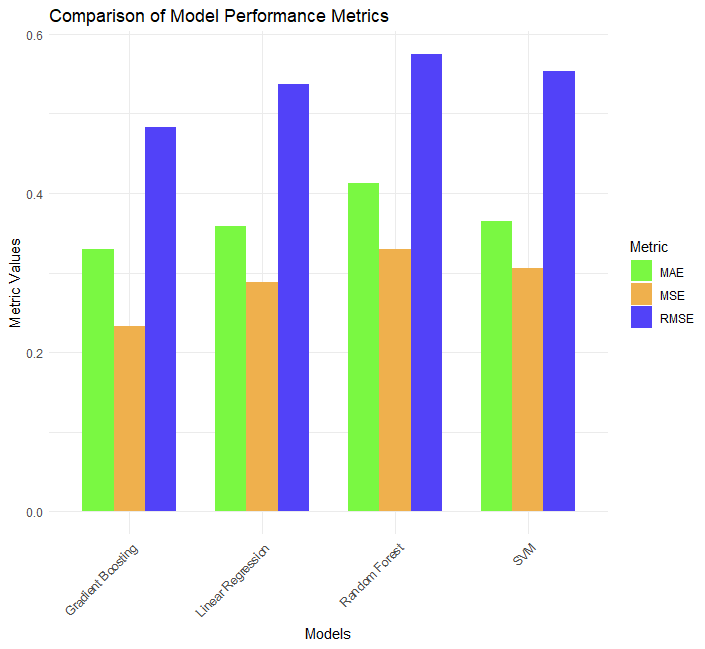
\includegraphics{Rplot.png}
\caption{Comparision of the model's evaluation metrics}
\end{figure}

\begin{figure}
\centering
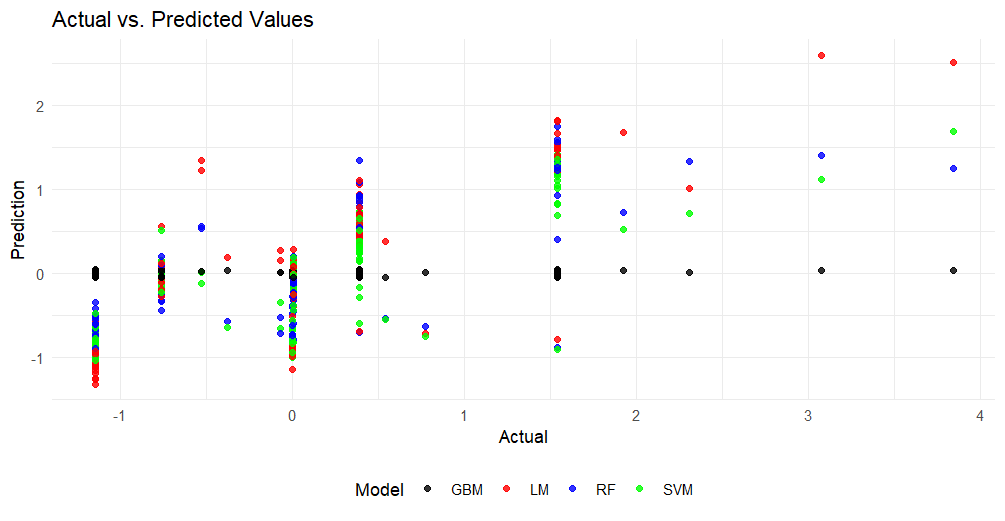
\includegraphics{idk.png}
\caption{Actual vs.~Predicted Values}
\end{figure}

The outcomes of the analysis highlight Gradient Boosting Regression as a
model with promising accuracy, potentially surpassing Linear Regression
in expense estimation. The observed marginally lower errors in Gradient
Boosting Regression suggest its ability to capture intricate patterns
within the dataset, potentially leading to improved predictions.
However, Linear Regression, while slightly less accurate, provided a
solid baseline for expense estimation among college students in urban
Saudi Arabia.

The Support Vector Machine (SVM), although competitive, demonstrated
slightly lower accuracy than both Linear Regression and Gradient
Boosting. The complexity of SVM might have slightly affected its
predictive capacity within this specific context. The hypothetical
exploration of Random Forest Regression hinted at potential
enhancements, yet empirical validation remains pivotal for establishing
its effectiveness in refining expense predictions. Summarize the key
findings from the analysis.

Addressing the limitations of the analysis is crucial. The study focused
primarily on a specific set of features related to expenses, potentially
overlooking other influential variables impacting students' spending
behaviors. Additionally, the availability and quality of data might have
influenced the models' performances. Future research should encompass a
wider spectrum of variables and gather more extensive, diverse datasets
to mitigate bias and enhance the models' robustness.

This investigation illuminates the potential of machine learning in
predicting monthly expenses among urban Saudi Arabian college students.
Gradient Boosting Regression stands out as a promising model, showcasing
marginally superior predictive accuracy. However, the theoretical
exploration of Random Forest Regression suggests untapped potential,
demanding empirical validation for conclusive insights.

\hypertarget{discussion}{%
\section{Discussion}\label{discussion}}

The exploration of college students' financial behaviors in urban Saudi
Arabia has been a critical endeavor, aimed at unraveling the intricate
patterns that shape spending habits within this unique cultural and
socioeconomic landscape. Throughout this research, our primary
objectives centered on comprehending the multifaceted influences on
spending patterns while acknowledging the challenges and limitations
inherent in such an analysis.

Our analysis, employing a range of statistical and machine learning
techniques, showcased promising outcomes in estimating monthly expenses
among college students. The models---Random Forest, Linear Regression,
SVM, and Gradient Boosting---demonstrated commendable accuracy,
revealing key predictors such as study year, living arrangements, and
major that significantly impact spending behaviors.

However, within the confines of our dataset and modeling approaches,
it's crucial to acknowledge the inherent limitations. While these models
offer valuable insights, they might not encapsulate the complete
spectrum of factors shaping individual spending behaviors. This
recognition lays the groundwork for potential avenues of improvement and
expansion in future research endeavors.

Our success lies not only in the creation of predictive models but also
in the identification of these limitations, which pave the way for
further investigations. Suggestions for feature engineering, model
refinement, and comprehensive data collection serve as pathways toward
enriching our understanding of the complex dynamics influencing student
spending behaviors.

Moving forward, a deeper exploration of nuanced factors like
extracurricular activities, family income, or social habits could
contribute to a more comprehensive understanding of student financial
dynamics. Additionally, refining models and exploring advanced
methodologies could enhance predictive accuracy and broaden the
applicability of our findings.

In conclusion, this research has provided significant insights into the
financial behaviors of college students in urban Saudi Arabia. It not
only highlights the potential of machine learning techniques in
estimating expenses but also underscores the necessity for continuous
refinement and expansion of research parameters to truly comprehend the
intricate web of factors influencing spending habits. This study sets
the stage for future investigations and practical applications aimed at
tailored support systems and business strategies catering to the
specific needs of Saudi college students.

\hypertarget{references}{%
\section{References}\label{references}}

Al, S. S., \& Abu. (2023). Factors Influencing Consumer Behavior towards
Online Shopping in Saudi Arabia Amid COVID-19: Implications for
E-Businesses Post Pandemic. Journal of Risk and Financial Management,
16(1), 36--36. \url{https://doi.org/10.3390/jrfm16010036}

Al-Khateeb, E., Al-Khateeb, B., \& Algharabat, R. (2015). Saudi
consumers' behaviors towards the use of credit cards. International
Journal of Bank Marketing, 33(4), 423-440.

Al-Rethaiaa, A. S., Fahmy, A.-E. A., \& Alshwaiyat, N. M. (2010).
Obesity and eating habits among college students in Saudi Arabia: a
cross sectional study. Nutrition Journal, 9(1).
\url{https://doi.org/10.1186/1475-2891-9-39}

Ali Saleh Alshebami, \& Theyazn H. H. Aldhyani. (2022). The Interplay of
Social Influence, Financial Literacy, and Saving Behaviour among Saudi
Youth and the Moderating Effect of Self-Control. Sustainability, 14(14),
8780--8780. \url{https://doi.org/10.3390/su14148780}

Alsahafi, N., \& Shin, S.-C. (2017). Online. Journal of International
Students, 7(1), 53--72. Retrieved from
\url{https://files.eric.ed.gov/fulltext/EJ1125725.pdf}

Ben Douissa, I. (2020, November). Factors affecting college students'
multidimensional financial literacy in the Middle East. International
Review of Economics Education.
\url{https://www.sciencedirect.com/science/article/abs/pii/S1477388019300611}

Hamdan, A., Sue L.T. Mcgregor, \& Elhassan, W. (2021, June 5). Financial
Literacy, Stability, and Security as Understood by Male Saudi University
Students. Retrieved December 14, 2023, from ResearchGate website:
\url{https://www.researchgate.net/publication/352251201_Financial_Literacy_Stability_and_Security_as_Understood_by_Male_Saudi_University_Students}

Otaibi, A., \& Kausar Yasmeen. (2014, December). Saudi consumer's
shopping behaviour: Descriptive Analysis. Retrieved December 14, 2023,
from ResearchGate website:
\url{https://www.researchgate.net/publication/287531379_Saudi_consumer\textquotesingle{}s_shopping_behaviourDescriptive_Analysis}

Qahwaji, D. M. (2023). Lifestyle behaviours, dietary habits, physical
activity and biochemical measurements in Saudi University students.
Medical Science, 27(134).
\url{https://doi.org/10.54905/disssi/v27i134/e198ms2940}

Rehr, T., Regan, E., \& Abukar, Z. (2022, March). Financial Wellness of
first-generation college students - researchgate.
\url{https://www.researchgate.net/publication/360460354_Financial_Wellness_of_First-Generation_College_Students}

Saeed, T. (2014, October 13). Examining the Level of Financial Literacy
among Saudi Investors and Its Impact on Financial Decisions. Retrieved
December 14, 2023, from ResearchGate website:
\url{https://www.researchgate.net/publication/287399490_Examining_the_Level_of_Financial_Literacy_among_Saudi_Investors_and_Its_Impact_on_Financial_Decisions}

\hypertarget{appendix}{%
\section{Appendix}\label{appendix}}

\end{document}
